This chapter is devoted to the evaluation of Particle Q Learning on classic benchmark problems, both in the tabular and in the function approximation cases. In Section ~\ref{sec:tabular_experiments} we show the results of experiments in the tabular case for classic problems found in the literature. Section ~\ref{sec:atari_experiments} describes the experiments performed in the \emph{Arcade Learning Environment} (ALE) ~\cite{Bellemare:2013:ALE:2566972.2566979}, a classic benchmark in the Deep RL literature. 
\section{Tabular Case} \label{sec:tabular_experiments}
This section is devoted to experiments conducted in finite domains where the tabular version of the algorithm can be used. The experiments are done in 6 different domains taken from the literature on efficient and deep exploration. Combining  the two policies (VPI policy and Weighted Policy) with the two update methods (Maximum Mean Updating and Weighted Updating) proposed in the previous Chapter we propose four versions of Particle Q-learning. We compare the results produced using these algorithms with the ones produced from different variations of two algorithms from the literature:
\begin{itemize}
\item Q-learning with $\epsilon$-greedy or Boltzman exploration,
\item Bootstrapped Q-learning with the Bootstrapped policy defined in ~\cite{DBLP:journals/corr/OsbandBPR16} and with the Weighted policy discussed in the previous chapter.
\end{itemize}
For all algorithms we have also considered their ``double'' versions, \ie modifications of the algorithms that use two Q-tables as in ~\cite{Hasselt:2016:DRL:3016100.3016191}. 
\subsection{Evaluation Metrics}
In this thesis, we addressed the exploration vs. exploitation dilemma by maintaining Q-distributions and using them to perform more informed decisions. A reinforcement learning agent needs exploration to learn an optimal policy faster in complex domains, but also not to get stuck in sub-optimal policies in domains that except them, and where discovering the optimal policy might be ``trickier''. For this purpose we test our algorithms in 6 domains, some of them designed to be ``tricky'', and some classical navigation problems. We compare algorithms by looking at the learning curve, \ie mean scores collected as a function of the training time. Algorithms that explore better, should not only show faster increasing curves, but also not get stuck in sub-optimal solutions. We show the mean scores over multiple runs, by shadowing around the curves to show also 95\% confidence interval.\par
We will also discuss how the Q-distributions maintained by the agent progress during learning. As we mentioned in the previous Chapter, as learning continues, the distributions should shrink to the true Q-value. We note that if the distributions shrink too quick, the agent might be stuck in a suboptimal policy. For this purpose we will show the following:
\begin{itemize}
\item Particle positions as learning progresses, to see if they do in fact converge,
\item Variance of the Q-distributions, which should converge to 0,
\item Probability of exploration, \ie probability of choosing an action different than the greedy one.
\end{itemize}
The first two of these curves are defined for each $(s,a)$ pair, whereas the last curve is defined for each state.
\subsection{Chain Domain}
The first domain we describe, taken from~\cite{Dearden98bayesianq-learning}, is shown in Figure ~\ref{fig:chain_domain}. The domain is composed of 5 states, labeled from 1 to 5. The agent can choose between two actions in each domain, labeled as $a$, $b$ (represented in the figure as the edges). The labels in the edges represent the action executed and the reward collected from the transition. With probability $p=0.2$ each action ``fails'' and the opposite action is executed instead, \ie we observe reward $r$ and next-state $s'$ of the opposite action. The domain is designed to test exploration approaches. Assuming a discount factor $\gamma=0.99$, the optimal policy is to always execute action $a$ to receive the high reward at the last state. If the agent does not explore enough it could be stuck in the suboptimal policy of executing always $b$ and collecting the smaller reward of 2.
\begin{figure}
 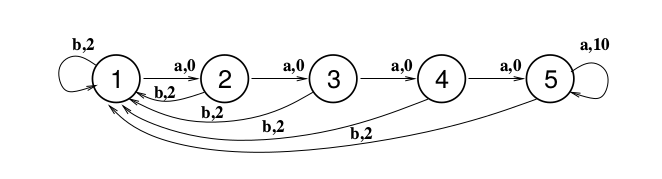
\includegraphics[width=\linewidth]{chain_domain.png}
 \caption{Chain domain taken from ~\cite{Dearden98bayesianq-learning}.}
 \label{fig:chain_domain}
\end{figure}
\subsection{Loop Domain}
The second domain we consider, shown in Figure ~\ref{fig:loop_domain}, is also taken from~\cite{Dearden98bayesianq-learning}. Similar to the first domain, the agent has 2 available actions in each of the 9 states. The name comes from the fact that, starting from the initial state 0, the agent has to choose between the two loops available. All rewards are 0, except the last transitions of the loops. The agent has to learn to perform the left loop, which gives the highest reward, but the right loop, although suboptimal, is easier to reach. An agent that does not explore enough might be stuck in the suboptimal loop.
\begin{figure}
 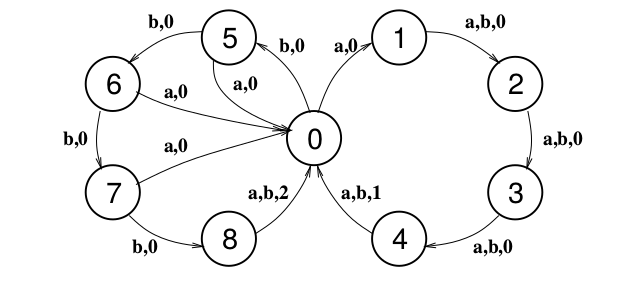
\includegraphics[width=\linewidth]{loop_domain.png}
 \caption{Loop domain taken from ~\cite{Dearden98bayesianq-learning}.} ~
 \label{fig:loop_domain}
\end{figure}
\subsection{Taxi Domain}
We will now review our results in the Taxi domain. This is domain is a classical benchmark for exploration in literature and has different versions. We will consider the version taken from \cite{Dearden98bayesianq-learning} where it appears as the Maze domain. The domain is shown in Figure ~\ref{fig:taxi_domain}.\par 
Taxi is a navigation problem. The environment is a $5\times5$ grid with 5 special locations labeled by different letters (S,F,F,F,G). The agent starts from cell $S$ (start). The objective of the agent is to pick up passengers, situated at the F (flag) locations and drop them off at the goal location (G). The reward is zero for every transition except when the goal is reached, where the reward collected depends on the number of passengers the agent has picked up. When the agent reaches the goal, the reward is 0, 1, 3, 15 for 0, 1, 2 and 3 passengers collected respectively.\par 
The agent has 4 possible actions, up, down, left and right. The agent picks up passengers by going in their location, but does not observe the reward until it reaches the goal state. The environment also has walls in some locations. When an agent performs an action that would transition into a location occupied from a wall, the agent does not change its location. Finally, each action has a 0.1 probability of ``failing''. When an action fails, the agent goes in a perpendicular direction instead. The challenge of the domain is to do sufficient exploration and collect all passengers before going to the goal.
\begin{figure}
 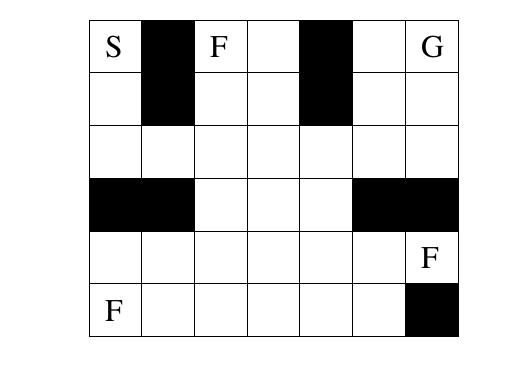
\includegraphics[width=\linewidth]{taxi_domain.png}
 \caption{Taxi domain taken from ~\cite{Dearden98bayesianq-learning}, where it appears as the Maze domain.} ~
 \label{fig:taxi_domain}
\end{figure}
\subsection{River Swim Domain }
The next domain we consider is the River Swim domain, taken from ~\cite{Strehl2008AnAO}. The environment is shown in Figure ~\ref{fig:riverswim_domain}. The MDP consists of six states numbered 1 to 6. The two actions available to the agent are to swim left or right represented by the edges in the figure. The agent starts in one of the states near the beginning of the row. Swimming to the right (against the current of the river) will more often than not leave the agent in the same state, but will sometimes transition the agent to the right (and with a much smaller probability to the left). Swimming to the left (with the current) always succeeds in moving the agent to the left, until the leftmost state is reached at which point swimming to the left yields a small reward of five units. The agent receives a much larger reward, of ten thousand units, for swimming upstream and reaching the rightmost state. The $(a,p,r)$ labels next to the edges in Figure~\ref{fig:riverswim_domain} represent the action, probability of success and reward tuple. For example, the label (1,0.7,0) next to the edge from node 0 to node 0 means that when executing action 1 from state 0 there is a 0.7 probability of staying in node 0 and receiving reward 0 and a 0.3 probability of transitioning to state 1 and receiving again reward 0.
\begin{figure}
 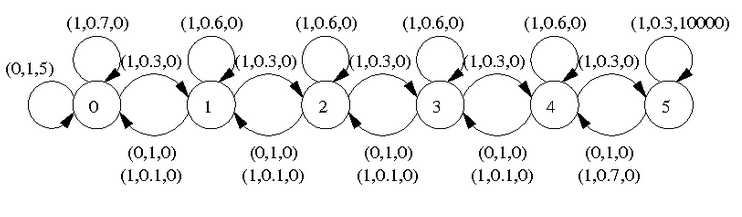
\includegraphics[width=\linewidth]{riverswim_domain.png}
 \caption{River Swim domain taken from ~\cite{Strehl2008AnAO}.} ~
 \label{fig:riverswim_domain}
\end{figure}
\subsection{Six Arms Domain}
The next environment is again taken from ~\cite{Strehl2008AnAO}. Six Arms, shown in Figure ~\ref{fig:sixarms_domain}, consists of seven states, one of which is the initial state. For how it is build, Six Arms resembles a multi armed bandit problem. The agent must choose from six different actions. Each action pulls a different arm, with a different payoff probability. When the arm pays off, the agent is sent to another state. Within that new state, large rewards can be obtained. The higher the payoff probability for an arm, the smaller the reward received (from the room the agent is sent to by the arm). In this MDP, a decision maker can make use of smaller amounts of experience on the low paying arms and still perform well.
\begin{figure}
 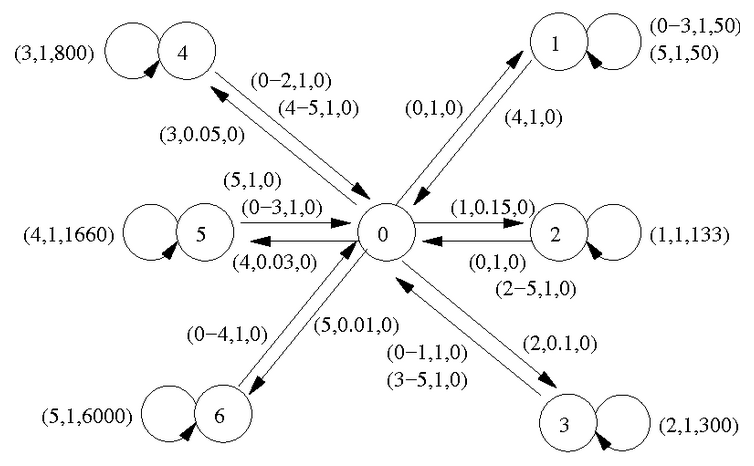
\includegraphics[width=\linewidth]{sixarms_domain.png}
 \caption{Six Arms domain taken from ~\cite{Strehl2008AnAO}.} ~
\label{fig:sixarms_domain}
\end{figure}
\subsection{Knight Quest}
The last environment we will test our algorithm in is called Knight Quest~\cite{DBLP:conf/icml/FruitPLO18}. This environment takes inspiration from classical arcade games. The goal is to rescue a princess in the shortest time without being killed by the dragon. To achieve this task, the knight needs to collect gold, buy the magic key and reach the princess location. A representation of the game is given in Figure ~\ref{fig:knightquest_domain}.\par
\begin{figure}
 \centering 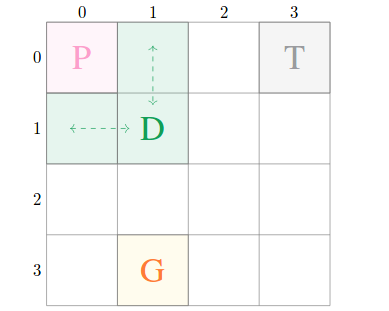
\includegraphics[width=10cm]{knightquest_domain.png}
 \caption{Knight Quest domain taken from ~\cite{DBLP:conf/icml/FruitPLO18}. The green cells are the three locations the dragon can move to.} ~
\label{fig:knightquest_domain}
\end{figure}
The elements of the game are:
\begin{itemize}
\item The knight,
\item the princess,
\item the dragon patrolling the princess,
\item a gold mine,
\item a town.
\end{itemize}
The knight is the only player of the game. He moves in the environment using the four cardinal actions (\ie right, down, left and up) plus an action to keep the current position (stay). Additionally, the knight can collect the gold (collect gold), buy a key (buy key) or buy an armour (buy armour).\par
The town (T) is the place where the knight can buy objects and where it is reset when he rescues the princess or he is killed by the dragon. Saving the princess (P) is the objective, while the gold mine (G) is the place where the knight can collect gold. The dragon (D) is the enemy and it is randomly moving around the princess's location. The dragon can kill the knight when they are at the same position and the knight does not have the armour. We denote as $d \in \{0,1,2\}$ the position of the dragon such that: $d = 0 := (0,1)$, $d= 1 := (1,0)$ and $d= 2 := (1,1)$. The transition probabilities of the dragon are:
\begin{equation*}
p_d(\cdot \vert 0)=[0.4,0,0.6]; \qquad p_d(\cdot \vert 1)=[0,0.4,0.6]; \qquad p_d(\cdot \vert 2)=[0.4,0.2,0.4]. 
\end{equation*}
\par
The state $s_t$ of the game is represented by the following elements:
\begin{itemize}
\item Knight position: coordinates of the grid, $(row,col), \quad row,col \in \{0,1,2,3\};$
\item Gold level: the amount of gold own by the knight, $g \in \{0,1\}$;
\item Dragon position: $d \in \{0,1,2\}$;
\item Object identifier: the object(s) owned by the knight, $o=\{0,1,2,3\}$ where 0 := nothing, 1 := key, 2 := armour and 3 :=key and armour.
\end{itemize}
The movement actions have the trivial effect of changing the knight position. The
action \emph{collect gold} changes the state only when the knight is at the mine. In this case the level of gold is incremented by one, formally $g_{t+1}= \min \{1,g_t + 1\}$. Actions \emph{buy key} and \emph{buy armour} alter the state only when are executed in the town with gold-level equal to 1. All the actions are deterministic when the knight does not own the armour. When the knight has the armour: 
\begin{itemize}
\item The movement actions result in a normal transition with probability 0.5, otherwise the current position is kept;
\item The \emph{collect gold} action fails with probability 0.9, \ie with probability 0.01 the gold level is increment by 1;
\item Actions \emph{buy key} and \emph{buy armour} are not modified.
\end{itemize}
When the knight is equipped with the armour it cannot be killed by the dragon (i.e., knight and dragon can occupy the same cell). At the same time, the armour makes the collection of the goal very challenging (i.e., success probability is 0.01).\par
The basic reward signal is $-1$ at each time step. Nevertheless, the knight receives a reward of $-10$ when he executes \emph{collect gold}, \emph{buy key} or \emph{buy armour} outside the designed location (i.e., mine and town).  The knight obtains a reward of $20$ when he reaches the princess with the key and $-20$ when he is killed by the dragon (i.e., knight and dragon are in the same cell and the knight
does not have the armour). Finally, when the episode ends (i.e., the knight reaches the princess with the key or he is killed), the knight is reset at town location with no gold or object ($g,o= 0$) and the dragon position is randomly drawn, $d \sim U(\{0,1,2\})$.
\section{Atari}		 \label{sec:atari_experiments}
In this section we will discuss the results of the ``deep'' version of our algorithm, Particle DQN, and compare its results with Bootstrapped DQN. We chose to compare our results with Bootstrapped DQN because both algorithms perform efficient and deep exploration using Q-distributions. Indeed the architecture of the deep network we use to conduct the experiments was taken from ~\cite{DBLP:journals/corr/OsbandBPR16}, which in turn adapts the famous DQN architecture designed by Mnih et al. in ~\cite{mnih2015humanlevel}.\par
We test our algorithms using the Arcade Learning Environment (ALE) described in ~\cite{Bellemare:2013:ALE:2566972.2566979}. Although there is a large number of Atari games we could have tested the algorithms, we present here results obtained in two games, due to the long training time required by the algorithm. It takes seven to eight days to train the agents in a single Atari game, this by considering training periods only half the length of the standard of the literature. This is further worsened by the fact that we had to run multiple instances of each algorithm in each environment to show the mean performance over multiple runs (a standard in literature to account for the random initialization of the deep networks).
\subsection{Experimental Setup}
Again we are testing for deep exploration, but in this section we focus in Atari games. Each step of the agent corresponds to four steps of the emulator, where the same action is repeated, the reward values of the agents are clipped between -1 and 1 for stability. We evaluate our agents and report performance based upon the raw scores and not the discounted scores. As it is common in literature, we do not show the online performance of the agent during training. We show the scores collected, when exploiting the greedy policies derived from the Q-function after each training period.\par
The \emph{convolutional} part of the network used is identical to the one used in ~\cite{DBLP:journals/corr/OsbandBPR16}. The input to the network is $4\times 84 \times 84$ \emph{tensor} with a rescaled, grayscale version of the last four observations. The first convolutional layer has 32 filters of size 8 with a stride of 4. The second layer has 64 filters of size 4 with stride 2. The last layer has 64 filters of size 3. We split the network beyond the final layer into $N = 20$ distinct heads, each one is fully connected and identical to the network in ~\cite{DBLP:journals/corr/OsbandBPR16}. This consists of a fully connected layer to 512 units followed by another fully connected layer to the Q-Values for each action. The fully connected layers all use \emph{Rectified Linear Units} (ReLU) as a \emph{non-linearity}. We normalize gradients $\frac{1}{N}$ that flow from each head as in ~\cite{DBLP:journals/corr/OsbandBPR16}.
We trained the networks with \emph{RMSProp} optimizer. The discount was set to $\gamma = 0.99$, the number of steps between target updates was set to $\tau= 10000$ steps. We trained the agents for a total of 25M steps per game, which corresponds to 100M frames. The agents were evaluated every 1M frames. \par
The \emph{experience replay} contains the 1m most recent transitions. We update the network every 4 steps by randomly sampling a minibatch of 32 transitions from the replay buffer to use the exact same minibatch schedule as Bootstrapped DQN. 